\documentclass{article}
\usepackage{geometry}
 \geometry{
 a4paper,
 total={170mm,257mm},
 left=20mm,
 top=20mm,
 }
\usepackage[english,greek, main=greek]{babel}
\usepackage[utf8]{inputenc}
\usepackage{amsmath}
\usepackage{graphicx} % for graphics and plots
\usepackage{subcaption} % for subfigures and subcaptions and \ContinuedFloat
\usepackage{placeins} % for \FloatBarrier
\usepackage{xcolor} % for colour definitions
\usepackage{listings} % for code highlighting
\usepackage{verbatim} % for file input
\usepackage{varwidth} % for centering verbatim 
\usepackage{hyperref} % clickable links
\usepackage{datatool} % for csv reading
\usepackage{tikz} % for tikz plot
\usetikzlibrary{datavisualization, babel} % for tikz plots

\newcommand{\eng}[1]{\foreignlanguage{english}{#1}} % shortcut for inserting english into greek text

\useshorthands{;}
\defineshorthand{;}{?} % greek question mark instead of english semicolon


\title{
    \includegraphics[width=\textwidth]{~/Pictures/emp.png} \\
    \vskip 5cm
    Κατανεμημένα Συστήματα \\
    \large Εξαμηνιαία Εργασία - \eng{BlockChat} 
    \vskip 5cm
}

\author{ Αναστάσιος Στέφανος Αναγνώστου \\ \large 03119051 }

\begin{document}

\maketitle \clearpage \tableofcontents \clearpage

\part{Σχεδιασμός Συστήματος}

\section{Δεν είμαι σίγουρος}

\clearpage
\part{Πειράματα}

Ανά πείραμα αξιολογούνται, αφενός τα πιο χρονοβόρα κομμάτια του κώδικα, όπως
υποδεικνύει το \eng{profiling} καθενός κόμβου κατά την εκτέλεση του πειράματος,
αφετέρου οι συναρτήσεις \eng{mint}, \eng{validateTransaction} και
\eng{processTXs}, οι οποίες συνιστούν την λογική λειτουργίας των κόμβων του
συστήματος. Επίσης, εκτιμάται η ρυθμαπόδοση του συστήματος και το μέσο
\eng{block time}.

\section{Απόδοση του συστήματος}

Σημειώνεται ότι το ποσοστό του χρόνου εκτέλεσης των σημείων που υποδεικνύει το
\eng{profiling} δεν είναι κληρονομημένο, δηλαδή δεν εμπεριέχονται στο ποσοστό
οι χρόνοι εκτέλεσης των συναρτήσεων που καλούνται από τις συναρτήσεις που
εμφανίζονται στο \eng{profiling}.

\subsection{Χρονοβόρα τμήματα του κώδικα}

Στο πείραμα για την αξιολόγηση της ρυθμαπόδοσης του συστήματος, στήνεται ένα
δίκτυο 5 κόμβων, καθένας εκ των οποίων εκτελεί 1 \eng{staking}, με \eng{stake
10 BCC} συναλλαγή και 50 συναλλαγές (συγκεκριμένα αποστολές μηνυμάτων) προς
τους άλλους κόμβους. Η ταχύτητα αποστολής συναλλαγών είναι ίδια μεταξύ των
κόμβων, ίση με $10\frac{txs}{s}$ και παραμένει σταθερή μεταξύ όλων των
πειραμάτων.

Το πρώτο πράγμα που φαίνεται στο σχήμα \ref{fig:throughput-cost-centers} είναι
ότι το μακράν πιο χρονοβόρο μέρος του κώδικα είναι η συνάρτηση
\eng{modular\_exponentiation} που χρησιμοποιείται γενικά για την κρυπτογράφηση
/ αποκρυπτογράφηση και υπογραφή / επαλήθευση μηνυμάτων. Συγκεκριμένα, φαίνεται
να λαμβάνει περίπου το 50\% του συνολικού χρόνου εκτέλεσης του προγράμματος.

\graphicspath{{../experiments/profiled\_outputs/throughput_proper/}}

\begin{figure}[ht]
    \centering
    \begin{subfigure}{\textwidth}
        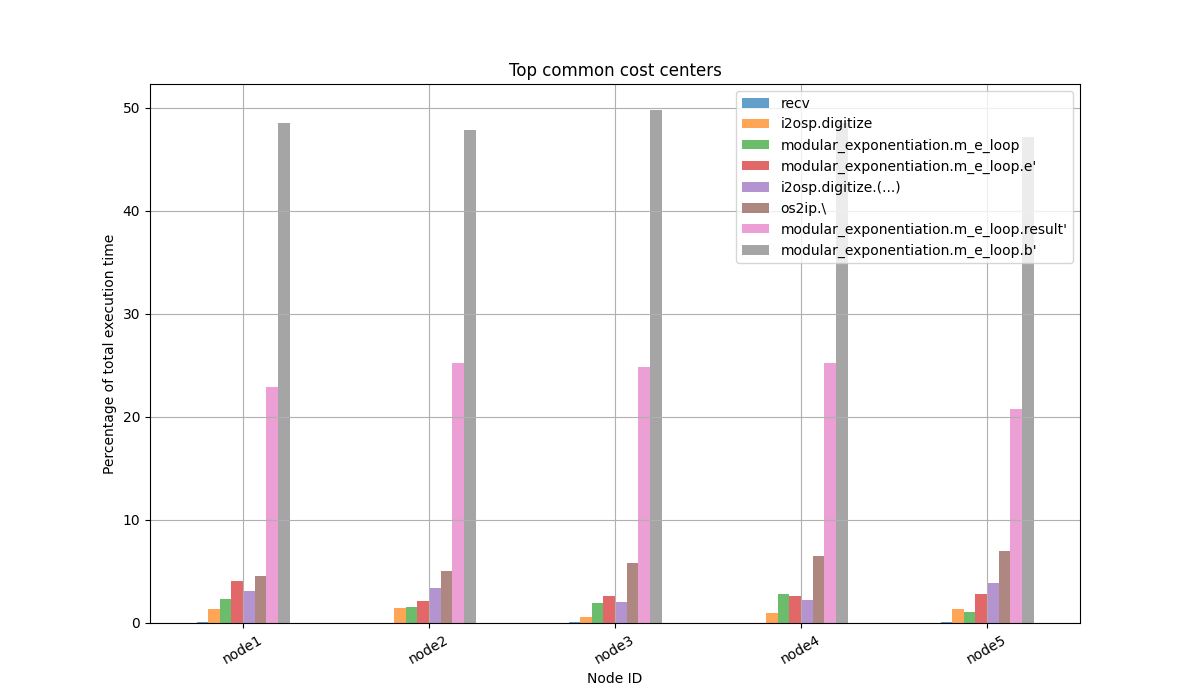
\includegraphics[width=\textwidth]{./capacity5/cost-centers-capacity5.png}
        \caption{\eng{capacity=5}}
    \end{subfigure}
\end{figure}
\begin{figure}[ht]
    \ContinuedFloat
    \begin{subfigure}{\textwidth}
        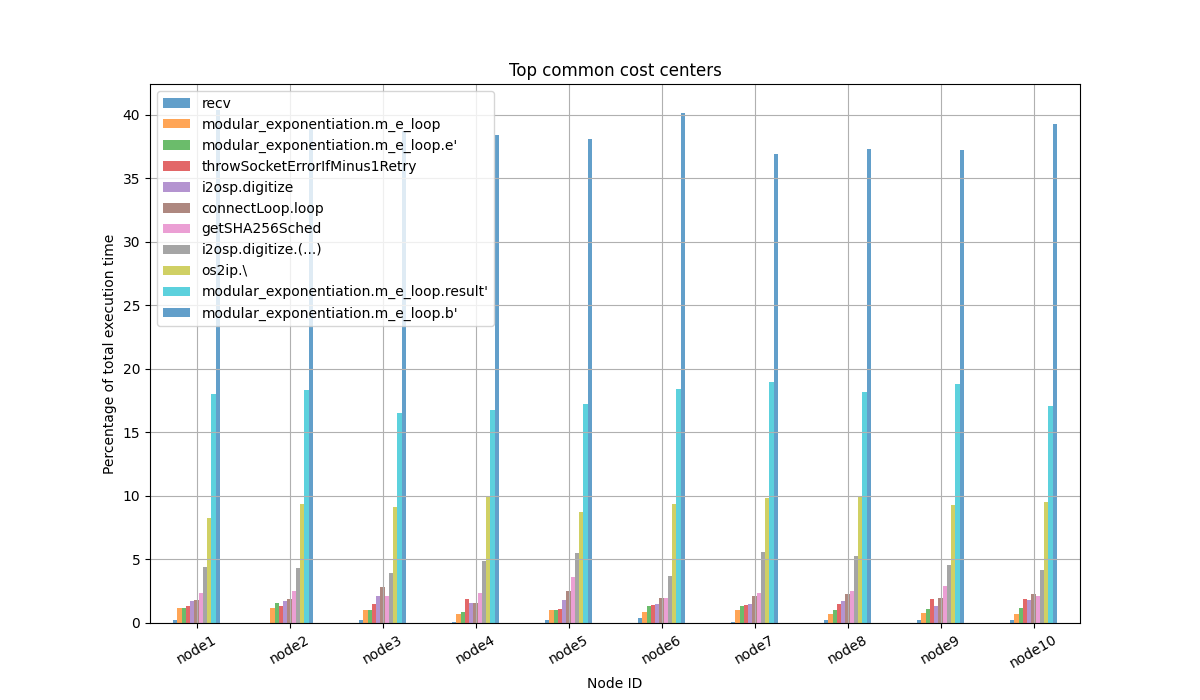
\includegraphics[width=\textwidth]{./capacity10/cost-centers-capacity10.png}
        \caption{\eng{capacity=10}}
    \end{subfigure}
    \begin{subfigure}{\textwidth}
        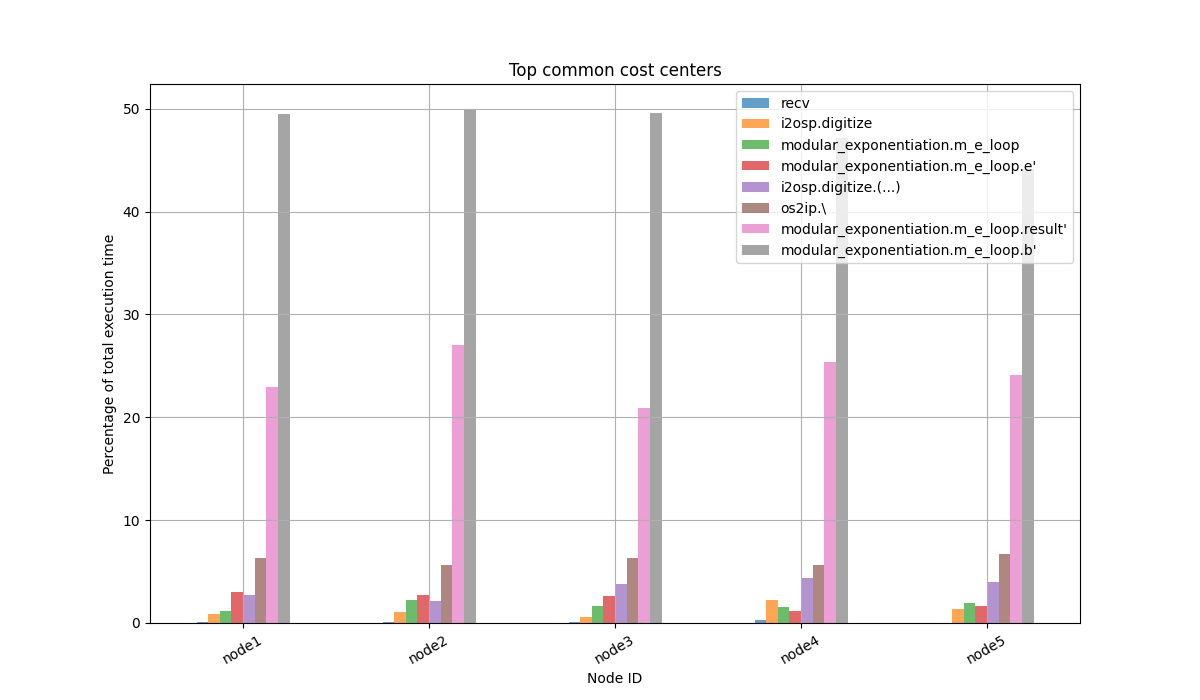
\includegraphics[width=\textwidth]{./capacity20/cost-centers-capacity20.png}
        \caption{\eng{capacity=20}}
    \end{subfigure}
    \caption{Τα πιο χρονοβόρα κομμάτια του κώδικα}
    \label{fig:throughput-cost-centers}
\end{figure}
\FloatBarrier

\subsection{Συναρτήσεις του συστήματος}

Σχετικά με τις \eng{top level} συναρτήσεις του συστήματος, παρατηρείται ότι, με
κάποιες μικρές διακυμάνσεις, η \eng{processTXs} καταναλώνει 9-10\% του
συνολικού χρόνου εκτέλεσης, η \eng{mint} 1-3\% και η \eng{validateTransaction}
7-9\%.

\begin{figure}[ht]
    \centering
    \begin{subfigure}{\textwidth}
        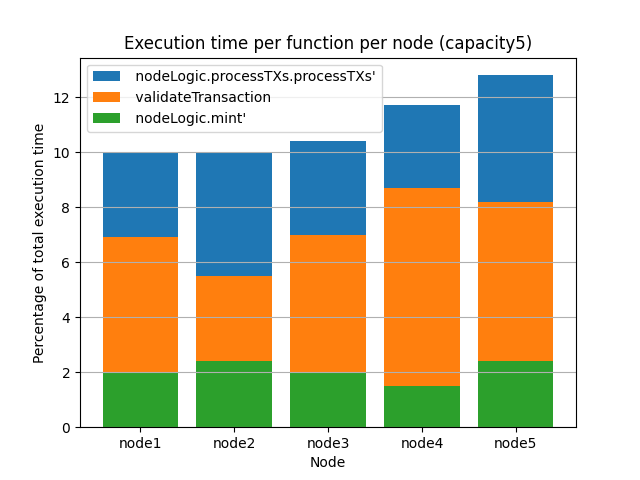
\includegraphics[width=\textwidth]{./capacity5/times_of_function_per_node_capacity5.png}
        \caption{Ρυθμαπόδοση \eng{capacity=5}}
    \end{subfigure}
\end{figure}
\begin{figure}[ht]
    \ContinuedFloat
    \begin{subfigure}{\textwidth}
        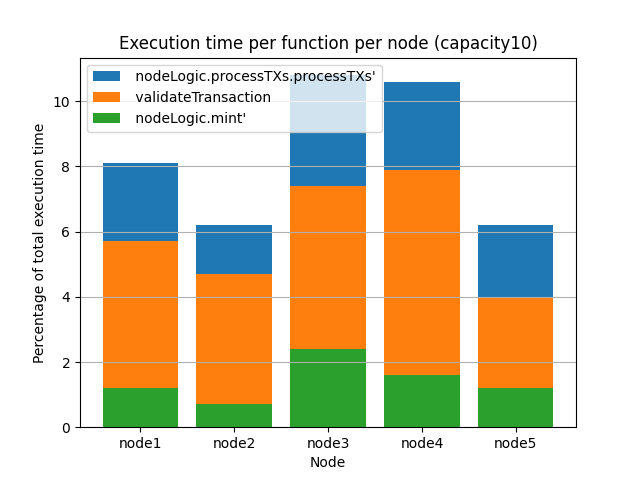
\includegraphics[width=\textwidth]{./capacity10/times_of_function_per_node_capacity10.png}
        \caption{Ρυθμαπόδοση \eng{capacity=10}}
    \end{subfigure}
    \begin{subfigure}{\textwidth}
        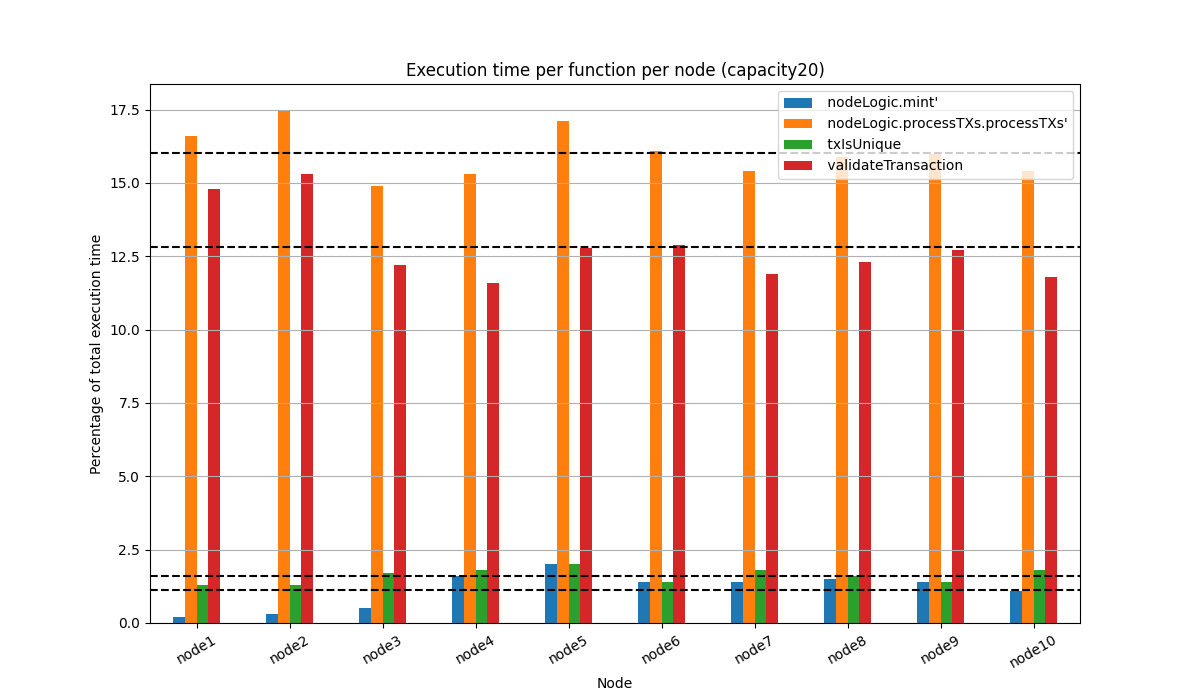
\includegraphics[width=\textwidth]{./capacity20/times_of_function_per_node_capacity20.png}
        \caption{Ρυθμαπόδοση \eng{capacity=20}}
    \end{subfigure}
    \caption{Ποσοστό χρόνου επί του συνολικού χρόνου εκτέλεσης που λαμβάνει η κάθε συνάρτηση}
\end{figure}
\FloatBarrier

Στον πίνακα \ref{tab:throughput-funcs} παρουσιάζονται ορισμένα στατιστικά
σχετικά με τις συναρτήσεις \eng{processTXs}, \eng{validateTransaction},
\eng{txIsUnique} και \eng{mint}. Το πιο σημαντικό να παρατηρηθεί είναι ότι, για
κάθε κόμβο, οι κλήσεις στην συνάρτηση \eng{validateTransaction} είναι ακριβώς
τόσες όσες και οι συναλλαγές που αποστέλλονται από όλους τους κόμβους $\left(5
+ 5 \times 50 = 255 \right)$. Επίσης, $\#mint + \#validateTransaction =
\#processTXs$ \footnote{Η -1 διαφορά είναι επειδή έγινε η τελευταία κλήση και τα
προγράμματα έλαβαν σήμα τερματισμού}. Παρ'ότι φαίνεται σαν να επικυρώθηκαν όλες
οι συναλλαγές, αυτό δεν ισχύει. Στην πραγματικότητα, επειδή οι κόμβοι δεν 
παραλαμβάνουν κατ'ανάγκην τις συναλλαγές με την σειρά αποστολή τους, είναι πιθανό
κάποιος \eng{validator} να ακυρώσει κάποια συναλλαγή η οποία με διαφορετική σειρά
θα είχε επιβεβαιωθεί. Για αυτόν τον λόγο φαίνεται ότι ένα υποσύνολο των συναλλαγών
εξετάζεται για την μοναδικότητά τους από την συνάρτηση \eng{txIsUnique}\footnote{Η
συνάρτηση είναι βέβαιο ότι επιστρέφει \eng{true} για όλες τις συναλλαγές, αφού
εκ κατασκευής είναι οι συναλλαγές μοναδικές}. Έτσι αιτιολογείται και το γεγονός
ότι το \eng{blockchain} έχει μήκος μικρότερο από το μέγιστο δυνατό του δεδομένων
των συναλλαγών. Παραδείγματος χάριν, για \eng{capacity 5} έχει μήκος 
$45 = \frac{228}{5} e \frac{255}{5} = 51$.

\DTLloaddb{th-calls1}{../experiments/profiled_outputs/throughput_proper/capacity5/calls-latex.csv}
\DTLloaddb{th-calls2}{../experiments/profiled_outputs/throughput_proper/capacity10/calls-latex.csv}
\DTLloaddb{th-calls3}{../experiments/profiled_outputs/throughput_proper/capacity20/calls-latex.csv}

\begin{table}[ht]
    \caption{Στατιστικά συναρτήσεων ανά κόμβο} 
    \label{tab:throughput-funcs}
    \begin{subtable}{\textwidth}
        \centering
        \caption{\eng{capacity=5}}
        \label{tab:throughput-funcs-1}
        \selectlanguage{english}
        \DTLdisplaydb{th-calls1}
        \selectlanguage{greek}
    \end{subtable}
\end{table}

\begin{table}[ht]
    \ContinuedFloat
    \begin{subtable}{0.45\textwidth}
        \centering
        \caption{\eng{capacity=10}}
        \label{tab:throughput-funcs-2}
        \selectlanguage{english}
        \DTLdisplaydb[MemInh]{th-calls2}
        \selectlanguage{greek}
    \end{subtable}
    \hfill
    \begin{subtable}{0.45\textwidth}
        \centering
        \caption{\eng{capacity=20}}
        \label{tab:throughput-funcs-3}
        \selectlanguage{english}
        \DTLdisplaydb[File,Function,MemInh]{th-calls3}
        \selectlanguage{greek}
    \end{subtable}
\end{table}
\FloatBarrier

\subsection{Ρυθμαπόδοση και \eng{Block time}}

Χρησιμοποιώντας τα στατιστικά από το \eng{profiling} καθενός κόμβου
μπορούν να εκτιμηθούν η ρυθμαπόδοση και το μέσο \eng{block time}.

\begin{figure}[ht]
    \begin{subfigure}{\textwidth}
        \centering
        \caption{\eng{capacity=5}}
        \label{fig:throughput-times-5}
        \selectlanguage{english}
        \begin{varwidth}{\linewidth}
            \verbatiminput{../experiments/profiled_outputs/throughput_proper/capacity5/final.csv}
        \end{varwidth}
        \selectlanguage{greek}
    \end{subfigure}
    \begin{subfigure}{\textwidth}
        \centering
        \caption{\eng{capacity=10}}
        \label{fig:throughput-times-10}
        \selectlanguage{english}
        \begin{varwidth}{\linewidth}
            \verbatiminput{../experiments/profiled_outputs/throughput_proper/capacity10/final.csv}
        \end{varwidth}
        \selectlanguage{greek}
    \end{subfigure}
    \begin{subfigure}{\textwidth}
        \centering
        \caption{\eng{capacity=20}}
        \label{fig:throughput-times-20}
        \selectlanguage{english}
        \begin{varwidth}{\linewidth}
            \verbatiminput{../experiments/profiled_outputs/throughput_proper/capacity20/final.csv}
        \end{varwidth}
        \selectlanguage{greek}
    \end{subfigure}
    \caption{Χρόνοι εκτέλεσης κόμβων}
    \label{fig:throughput-times}
\end{figure}
\FloatBarrier

Στον πίνακα \ref{tab:throughput-funcs} φαίνεται ότι, με εξαίρεση λίγους κόμβους
στο πείραμα χωρητικότητας 5, το δίκτυο φτάνει εντός πειράματος σε σταθερή κατάσταση,
έχοντας επαληθεύει όλες τις συναλλαγές.

\clearpage
\section{Κλιμακωσιμότητα του συστήματος}

Στο πείραμα κλιμακωσιμότητας, το δίκτυο εκκινείται με 10 κόμβους, καθένας εκ
των οποίων εκτελεί 1 \eng{staking} συναλλαγή, με \eng{stake 10 BCC} και 100
συναλλαγές (συγκεκριμένα αποστολές μηνυμάτων) προς τους άλλους κόμβους. Σκοπός
είναι να εξεταστεί η κλιμάκωση του συστήματος ως προς το πλήθος των
συμμετεχόντων κόμβων.

\subsection{Χρονοβόρα τμήματα του κώδικα}

Στα γραφήματα \ref{fig:scalability-cost-centers} φαίνονται τα πιο χρονοβόρα
κομμάτια του κώδικα για κάθε πείραμα κλιμακωσιμότητας. Φαίνεται ότι αυτά είναι
τα ίδια με τα πιο χρονοβόρα κομμάτια του κώδικα για το πείραμα ρυθμαπόδοσης, με
την συνάρτηση \eng{modular\_exponentiation} περίπου το 50\% του συνολικού
χρόνου εκτέλεσης του προγράμματος, αντί για το 40\% που ήταν προηγουμένως.

\graphicspath{{../experiments/profiled\_outputs/scalability_proper/}}

\begin{figure}[ht]
    \centering
    \begin{subfigure}{\textwidth}
        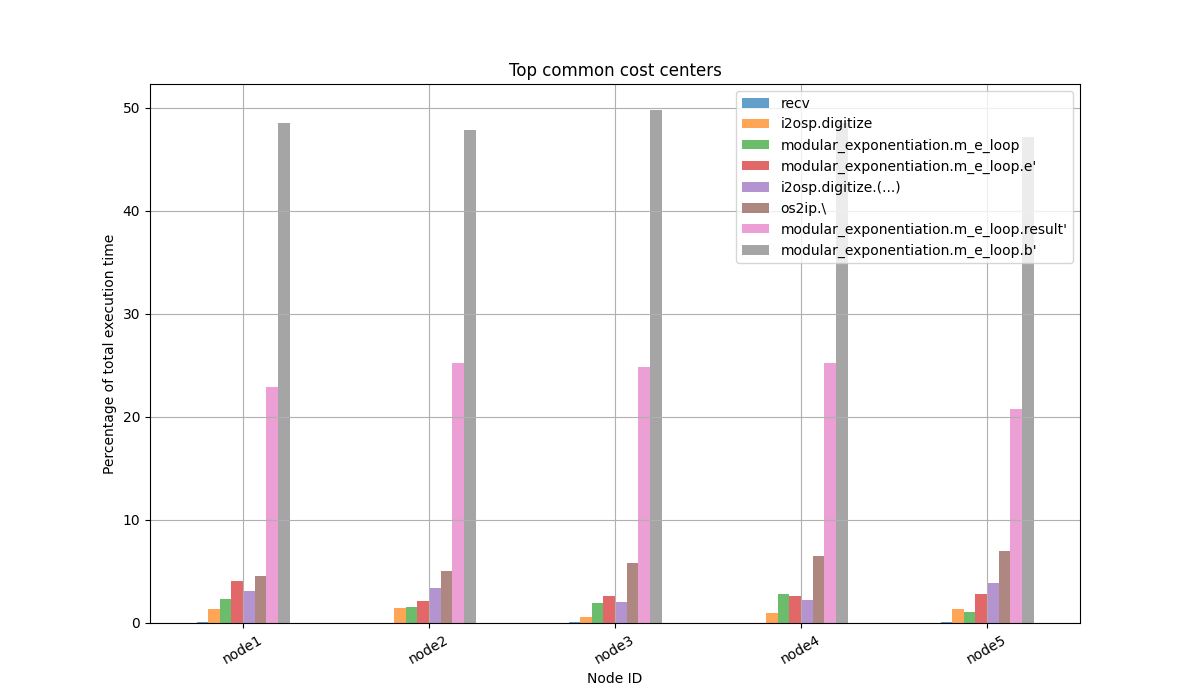
\includegraphics[width=\textwidth]{./capacity5/cost-centers-capacity5.png}
        \caption{\eng{capacity=5}}
    \end{subfigure}
\end{figure}
\begin{figure}[ht]
    \ContinuedFloat
    \begin{subfigure}{\textwidth}
        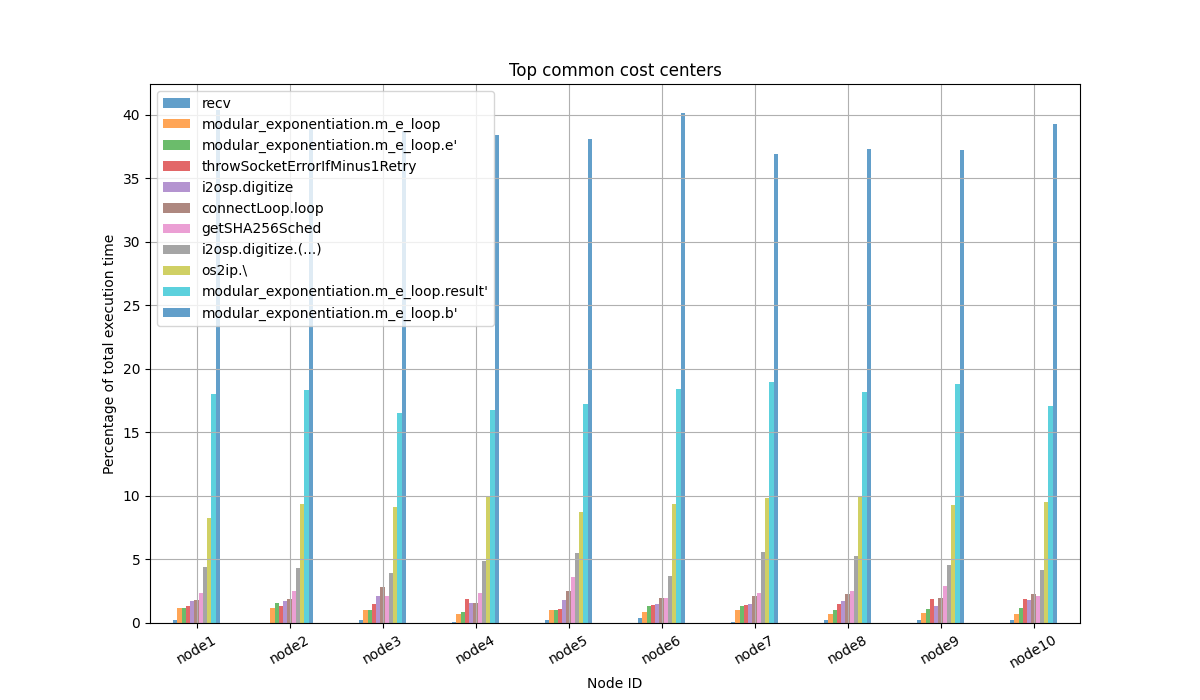
\includegraphics[width=\textwidth]{./capacity10/cost-centers-capacity10.png}
        \caption{\eng{capacity=10}}
    \end{subfigure}
    \begin{subfigure}{\textwidth}
        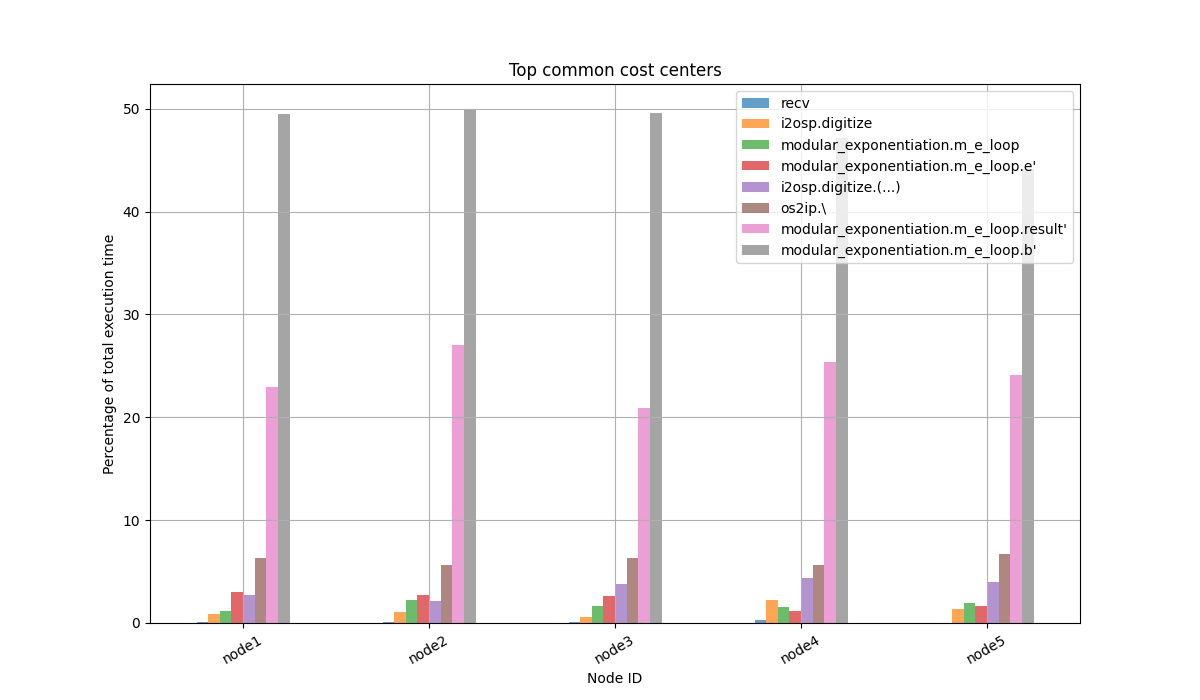
\includegraphics[width=\textwidth]{./capacity20/cost-centers-capacity20.png}
        \caption{\eng{capacity=20}}
    \end{subfigure}
    \caption{Τα πιο χρονοβόρα κομμάτια του κώδικα}
    \label{fig:scalability-cost-centers}
\end{figure}
\FloatBarrier

\subsection{Συναρτήσεις του συστήματος}

Αρχικά, στο γράφημα \ref{fig:scalability-funcs-5} αποτυπώνεται σαφώς το
γεγονός

Στα γραφήματα \ref{fig:scalability-funcs} παρατηρείται ότι η
\eng{validateTransaction} καταλαμβάνει περίπου 15\% του συνολικού χρόνου
εκτέλεσης, ενώ προηγουμένως κατελάμβανε περίπου 8\%. Δεδομένου ότι οι
συναλλαγές έχουν τετραπλασιαστεί, ο πολλαπλασιασμός του ποσοστού επί 2 φαίνεται
προβληματικός εκ πρώτης όψεως. Ωστόσο, ο χρόνος του τρέχοντος πειράματος είναι
διπλάσιος από τον χρόνο του προηγούμενου πειράματος, οπότε στην πραγματικότητα
ο χρόνος είναι ο τετραπλάσιος. Επομένως, ο χρόνος που ξοδεύει συνολικά ένας
κόμβος στην επικύρωση συναλλαγών αυξάνεται γραμμικά με το πλήθος των συμμετέχοντων
κόμβων, σε μία διάταξη όπως η παρούσα, όπου κάθε κόμβος στέλνει ένα σταθερό πλήθος
συναλλαγών ανά κόμβο.

\begin{figure}[ht]
    \centering
    \begin{subfigure}{\textwidth}
        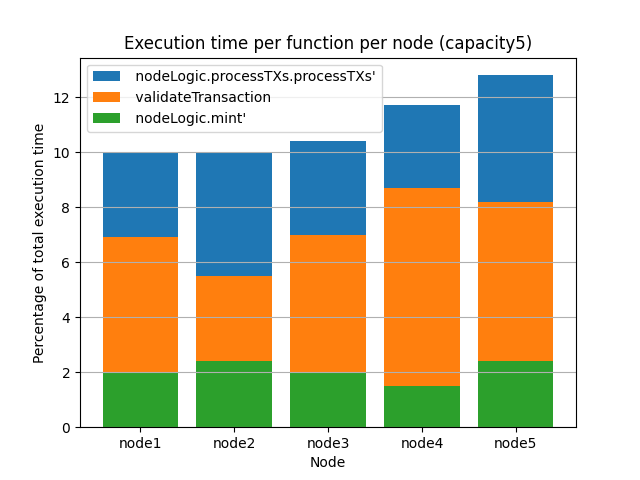
\includegraphics[width=\textwidth]{./capacity5/times_of_function_per_node_capacity5.png}
        \caption{\eng{capacity=5}}
        \label{fig:scalability-funcs-5}
    \end{subfigure}
\end{figure}
\begin{figure}[ht]
    \ContinuedFloat
    \begin{subfigure}{\textwidth}
        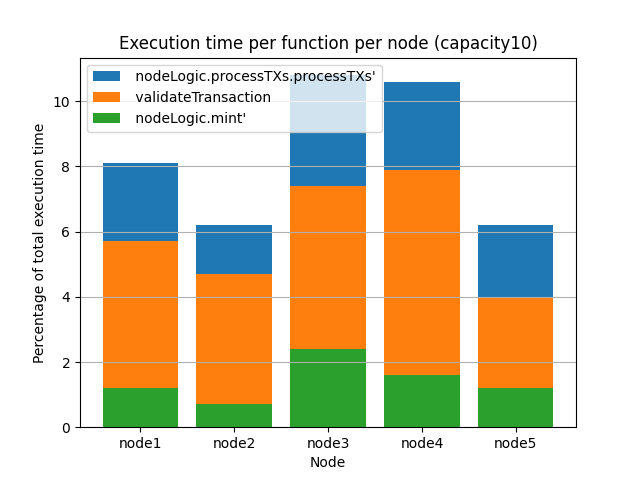
\includegraphics[width=\textwidth]{./capacity10/times_of_function_per_node_capacity10.png}
        \caption{\eng{capacity=10}}
        \label{fig:scalability-funcs-10}
    \end{subfigure}
    \centering
    \begin{subfigure}{\textwidth}
        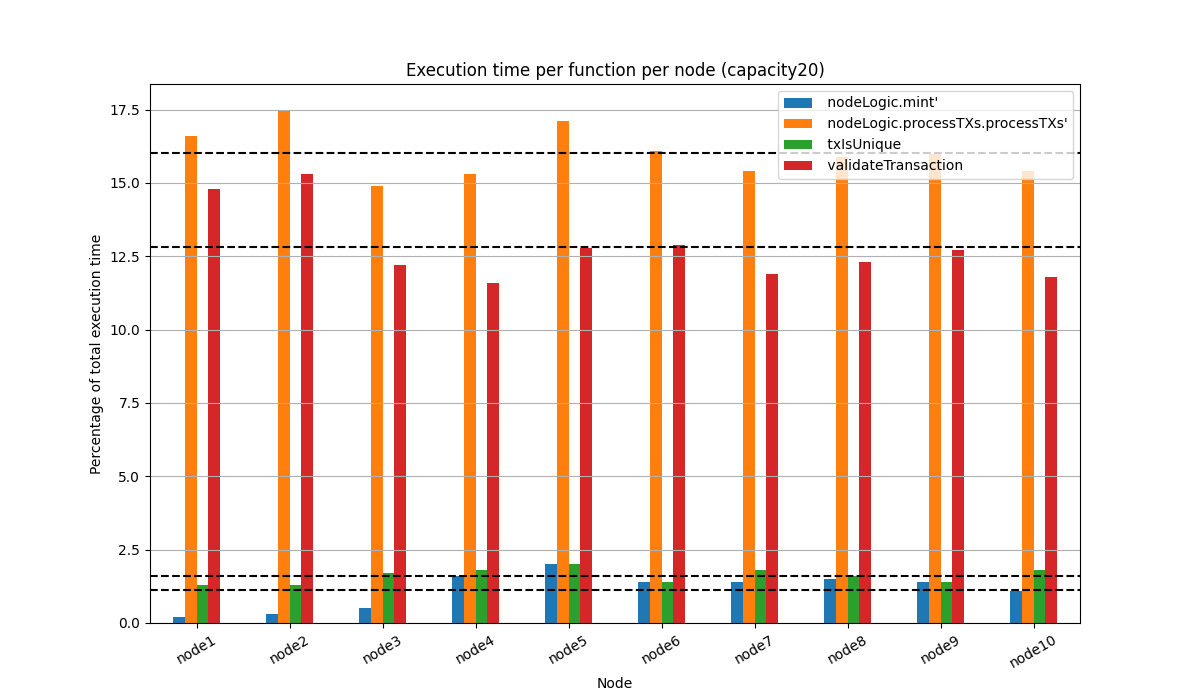
\includegraphics[width=\textwidth]{./capacity20/times_of_function_per_node_capacity20.png}
        \caption{\eng{capacity=20}}
        \label{fig:scalability-funcs-20}
    \end{subfigure}
    \caption{Ποσοστό χρόνου επί του συνολικού χρόνου εκτέλεσης που λαμβάνει η κάθε συνάρτηση}
    \label{fig:scalability-funcs}
\end{figure}
\FloatBarrier

\DTLloaddb{sc-calls1}{../experiments/profiled_outputs/scalability_proper/capacity5/calls-latex.csv}
\DTLloaddb{sc-calls2}{../experiments/profiled_outputs/scalability_proper/capacity10/calls-latex.csv}
\DTLloaddb{sc-calls3}{../experiments/profiled_outputs/scalability_proper/capacity20/calls-latex.csv}

Στον πίνακα \ref{tab:scalability-funcs-1} φαίνονται οι κλήσεις ενδιαφέροντος
των κόμβων. Παρατηρώντας το πλήθος των κλήσεων ανά συνάρτηση, διαπιστώνεται ότι
οι κόμβοι δεν προλαβαίνουν να επικυρώσουν όλες τις συναλλαγές που λαμβάνουν.
Αυτό οφείλεται, αφενός στον μεγαλύτερο όγκο συναλλαγών $10 + 10 \times 100 =
1010$ ο οποίος είναι $\approx 4$ φορές μεγαλύτερος από προηγουμένως, και
αφετέρου στην μικρή χωρητικότητα του \eng{block}, το οποίο σημαίνει ότι οι
κόμβοι πρέπει συχνά να καλούν την χρονοβόρα συνάρτηση \eng{mint} και να
διακόπτουν την διαδικασία επικύρωσης.

Επίσης, παρατηρείται ότι οι κόμβοι 7-8 έχουν μείνει πολύ πίσω σε σχέση
με τους υπόλοιπους κόμβους. Αυτό είναι μάλλον συνέπεια της πειραματικής
διάταξης, αφού όλοι οι κόμβοι τρέχουν στο ίδιο μηχάνημα.

\begin{table}[ht]
    \caption{Στατιστικά συναρτήσεων ανά κόμβο}
    \label{tab:scalability-funcs}
    \begin{subtable}{\textwidth}
        \centering
        \caption{\eng{capacity=5}}
        \label{tab:scalability-funcs-1}
        \selectlanguage{english}
        \DTLdisplaydb{sc-calls1}
        \selectlanguage{greek}
    \end{subtable}
\end{table}

Αντιθέτως, στους πίνακες \ref{tab:scalability-funcs-2} και \ref{tab:scalability-funcs-3}
φαίνεται από τις κλήσεις των συναρτήσεων ότι έχουν επικυρωθεί όλες οι συναλλαγές
και έχουν παραχθεί τα αντίστοιχα \eng{blocks}. Η μεγαλύτερη χωρητικότητα των
\eng{blocks} επιτρέπει στους κόμβους μεγαλύτερα χρονικά παράθυρα για την
επικύρωση των συναλλαγών και η διακοπή για την παραγωγή των \eng{blocks} δεν
καθυστερεί την εξέλιξη του δικτύου.

\begin{table}[ht]
    \ContinuedFloat
    \begin{subtable}{0.45\textwidth}
        \centering
        \caption{\eng{capacity=10}}
        \label{tab:scalability-funcs-2}
        \selectlanguage{english}
        \DTLdisplaydb[MemInh]{sc-calls2}
        \selectlanguage{greek}
    \end{subtable}
    \hfill
    \begin{subtable}{0.45\textwidth}
        \centering
        \caption{\eng{capacity=20}}
        \label{tab:scalability-funcs-3}
        \selectlanguage{english}
        \DTLdisplaydb[File,Function,MemInh]{sc-calls3}
        \selectlanguage{greek}
    \end{subtable}
\end{table}

Η ρυθμαπόδοση του συστήματος μπορεί να υπολογιστεί όπως προηγουμένως:

\begin{equation}
    \begin{gathered}
        \text{Ρυθμαπόδοση} = \frac{\text{Συνολικές συναλλαγές}}{\text{Συνολικός χρόνος}} \Rightarrow
        \left\{
            \begin{gathered}
                th_{capacity=5} = \frac{0.8 \times 62 + 0.2 \times 5}{10} \\
                th_{capacity=10} = \frac{1010}{10} \\
                th_{capacity=20} = \frac{1010}{10}
            \end{gathered}
        \right\} \Rightarrow \\
        \boxed{
            \begin{gathered}
                th_{capacity=5}  = 5.6\text{ }\frac{txs}{s} \\
                th_{capacity=10} = 101\text{ }\frac{txs}{s} \\
                th_{capacity=20} = 101\text{ }\frac{txs}{s}
            \end{gathered}
        }
    \end{gathered}
\end{equation}

Στο παρακάτω γράφημα φαίνεται η ρυθμαπόδοση του συστήματος για κάθε πείραμα:

\begin{figure}[h]
    \centering
    \caption{\eng{Throughput} του συστήματος}
    \label{fig:throughput-per-node}
    \selectlanguage{english}
    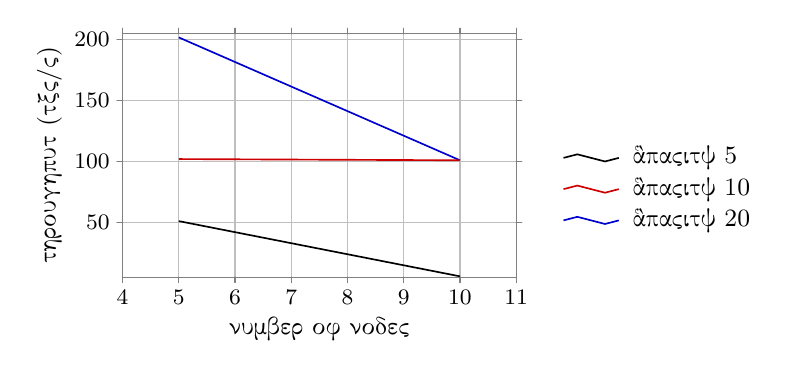
\begin{tikzpicture}
        \datavisualization [scientific axes, all axes={grid},
                            visualize as line/.list={capacity5, capacity10, capacity20},
                            x axis={label={number of nodes}, 
                                    min value=4, max value=11},
                            y axis={label={throughput (txs/s)},
                                    min value=5, max value=205},
                            capacity5={label in legend={text=Capacity 5}},
                            capacity10={label in legend={text=Capacity 10}},
                            capacity20={label in legend={text=Capacity 20}},
                            legend={right=0.5cm}, style sheet=strong colors,
                            ]
            data [set=capacity5] {
                x, y
                5, 51
                10, 5.6
            }
            data [set=capacity10] {
                x, y
                5, 102
                10, 101
            }
            data [set=capacity20]{
                x, y
                5, 202
                10, 101
            };
    \end{tikzpicture}
    \selectlanguage{greek}
\end{figure}
\FloatBarrier

\subsection{\eng{Block Time}}

Το μέσο \eng{block time} του συστήματος υπολογίζεται πάλι όπως προηγουμένως:

\begin{equation}
    \begin{gathered}
        \text{\eng{Block Time}} = \frac{\text{Συνολικός χρόνος}}{\text{Συνολικά \eng{blocks}}} \Rightarrow
        \left\{
            \begin{gathered}
                bt_{capacity=5} = \frac{0.8 \times 12 + 0.2 \times 1}{10} \\ 
                bt_{capacity=10} = \frac{50}{10} \\ 
                bt_{capacity=20} = \frac{0.1 \times 22 + 0.1 \times 23 + 0.8 \times 25}{10} \\
            \end{gathered} \right\}\Rightarrow \\ 
        \boxed{
            \begin{gathered}
                bt_{capacity=5} = 0.962\frac{blocks}{s} \\
                bt_{capacity=10} = 5\frac{blocks}{s} \\
                bt_{capacity=20} = 2.25\frac{blocks}{s}
            \end{gathered}
        }
    \end{gathered}
\end{equation}

\begin{figure}[h]
    \centering
    \caption{Μέσο \eng{block time} του συστήματος}
    \label{fig:block-time-per-node}
    \selectlanguage{english}
    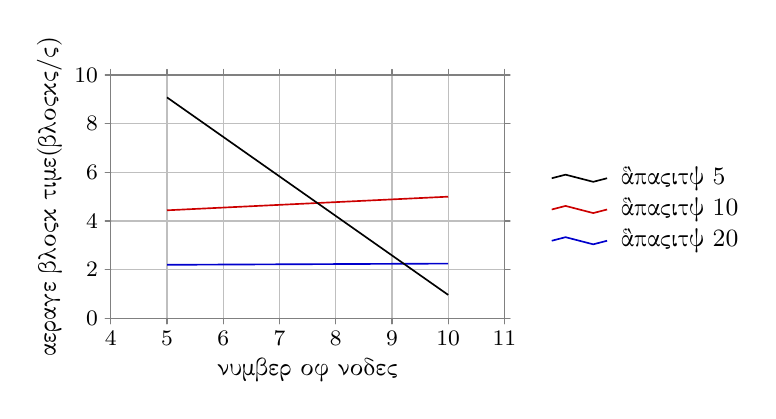
\begin{tikzpicture}
        \datavisualization [
            scientific axes, all axes={grid},
            visualize as line/.list={capacity5, capacity10, capacity20},
            x axis={label={number of nodes}, 
                    min value=4, max value=11},
            y axis={label={average block time(blocks/s)},
                    min value=0, max value=10},
            capacity5={label in legend={text=Capacity 5}},
            capacity10={label in legend={text=Capacity 10}},
            capacity20={label in legend={text=Capacity 20}},
            legend={right=0.5cm}, style sheet=strong colors,
        ]
            data [set=capacity5] {
                x, y
                5, 9.08
                10, 0.962
            }
            data [set=capacity10] {
                x, y
                5, 4.44
                10, 5
            }
            data [set=capacity20]{
                x, y
                5, 2.2
                10, 2.25
            };
    \end{tikzpicture}
    \selectlanguage{greek}
\end{figure}

\begin{figure}[ht]
    \begin{subfigure}{\textwidth}
        \centering
        \caption{\eng{capacity=5}}
        \label{fig:scalability-times-5}
        \selectlanguage{english}
        \begin{varwidth}{\linewidth}
            \verbatiminput{../experiments/profiled_outputs/scalability_proper/capacity5/final.csv}
        \end{varwidth}
        \selectlanguage{greek}
    \end{subfigure}
    \begin{subfigure}{\textwidth}
        \centering
        \caption{\eng{capacity=10}}
        \label{fig:scalability-times-10}
        \selectlanguage{english}
        \begin{varwidth}{\linewidth}
            \verbatiminput{../experiments/profiled_outputs/scalability_proper/capacity10/final.csv}
        \end{varwidth}
        \selectlanguage{greek}
    \end{subfigure}
    \begin{subfigure}{\textwidth}
        \centering
        \caption{\eng{capacity=20}}
        \label{fig:scalability-times-20}
        \selectlanguage{english}
        \begin{varwidth}{\linewidth}
            \verbatiminput{../experiments/profiled_outputs/scalability_proper/capacity20/final.csv}
        \end{varwidth}
        \selectlanguage{greek}
    \end{subfigure}
    \caption{Χρόνοι εκτέλεσης κόμβων}
    \label{fig:scalability-times}
\end{figure}
\FloatBarrier


\clearpage
\section{Δικαιοσύνη}

Στο πείραμα δικαιοσύνης, το δίκτυο εκκινείται με 5 κόμβους και ο υπ'αριθμόν 1
από αυτούς κάνει \eng{stake 100 BCC}, ενώ οι υπόλοιποι κάνουν \eng{stake 10 BCC}.

\graphicspath{{../experiments/profiled\_outputs/fairness_proper/}}
\begin{figure}[ht]
    \centering
    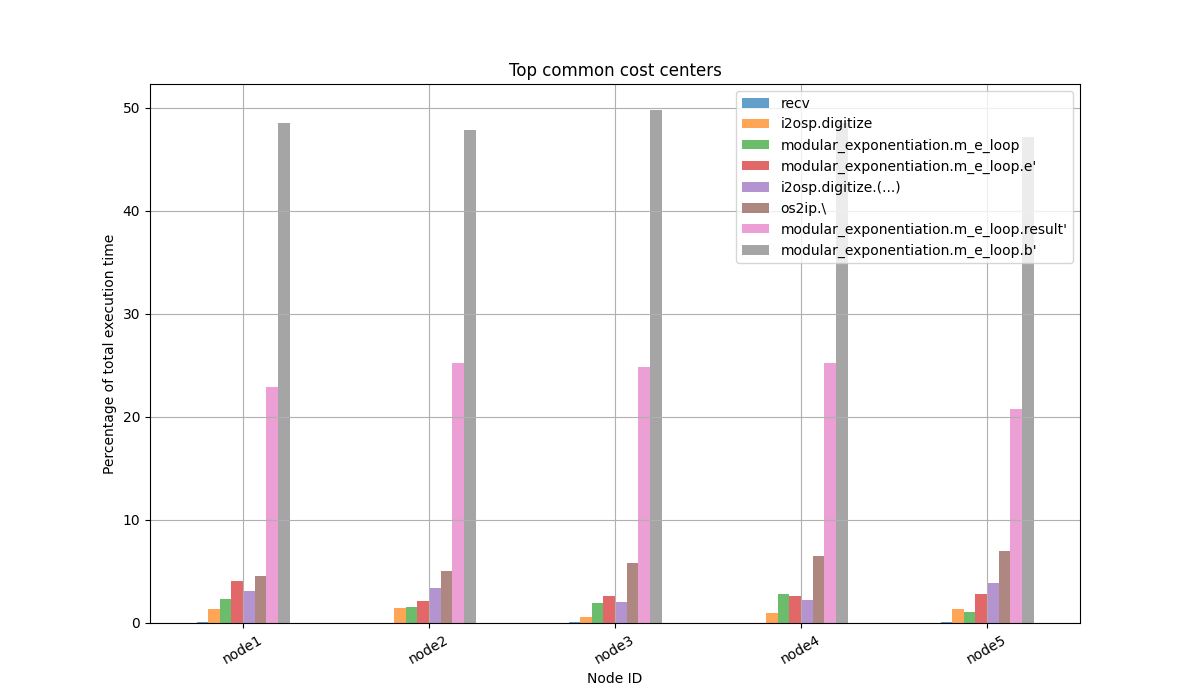
\includegraphics[width=\textwidth]{./capacity5/cost-centers-capacity5.png}
    \caption{Τα πιο χρονοβόρα κομμάτια του κώδικα \eng{capacity=5}}
    \label{fig:fairness-cost-centers}
\end{figure}

Στον πίνακα \ref{tab:fairness-funcs} φαίνονται οι κλήσεις μερικών συναρτήσεων
ενδιαφέροντος. Φαίνεται ότι τα πλήθη όλων των κλήσεων είναι ίδια ανά κόμβο,
πράγμα που σημαίνει ότι οι κόμβοι εκτελούν τις ίδιες λειτουργίες με την ίδια
συχνότητα. Παρ'όλα αυτά, ο κόμβος με το μεγαλύτερο \eng{stake} καταναλώνει πολύ
περισσότερο χρόνο στην συνάρτηση \eng{mint'} σε σχέση με τους υπόλοιπους
κόμβους, όπως φαίνεται και στο σχήμα \ref{fig:fairness-funcs}.

\DTLloaddb{fairness-calls}{../experiments/profiled_outputs/fairness_proper/capacity5/calls-latex.csv}
\begin{table}[ht]
    \centering
    \caption{Στατιστικά συναρτήσεων ανά κόμβο \eng{capacity=5}}
    \label{tab:fairness-funcs}
    \selectlanguage{english}
    \DTLdisplaydb{fairness-calls}
    \selectlanguage{greek}
\end{table}

\begin{figure}[ht]
    \centering
    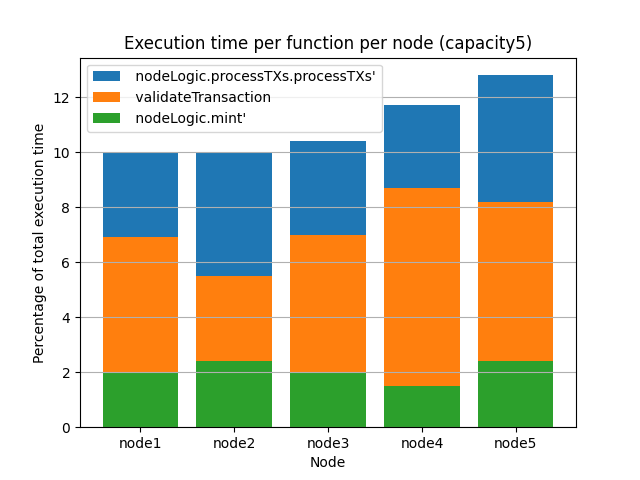
\includegraphics[width=\textwidth]{./capacity5/times_of_function_per_node_capacity5.png}
    \caption{Ποσοστό χρόνου επί του συνολικού χρόνου εκτέλεσης που λαμβάνει η κάθε συνάρτηση \eng{capacity=5}}
    \label{fig:fairness-funcs}
\end{figure}
\FloatBarrier

Στο σχήμα \ref{fig:fairness-funcs} φαίνεται, πράγματι, ότι ο κόμβος με το
μεγαλύτερο \eng{stake} καταναλώνει πολύ περισσότερο χρόνο στην συνάρτηση
\eng{mint'} σε σχέση με τους υπόλοιπους κόμβους, ενδεικτικό του γεγονός ότι
πράγματι αυτός αναλαμβάνει συχνότερα την δημιουργία των νέων \eng{blocks}.
Μάλιστα, επισκοπώντας τα υπόλοιπα των λογαριασμών των κόμβων στο σχήμα
\ref{fig:fairness-balances}, παρατηρεί κανείς ότι όντως τα περισσότερα
νομίσματα συσσωρεύονται στον κόμβο με το μεγαλύτερο \eng{stake}.

\begin{figure}[h]
    \centering    
    \selectlanguage{english}
    \begin{varwidth}{\linewidth}
        \verbatiminput{../experiments/profiled_outputs/fairness_proper/capacity5/balances.out}
    \end{varwidth}
    \selectlanguage{greek}
    \caption{Υπόλοιπα λογαριασμών κόμβων \eng{capacity=5}}
    \label{fig:fairness-balances}
\end{figure}

\end{document}
